% =====================================================================
% Relatório Final - Projeto de Extensão
% Uso da Inteligência Artificial em Aplicações Computacionais (UTFPR)
% Jogo "Guardiões da Energia"
% Compilar com pdfLaTeX (ex.: Overleaf). As figuras ficam na pasta figuras/.
% =====================================================================
\documentclass[12pt,a4paper]{article}

\usepackage[utf8]{inputenc}
\usepackage[T1]{fontenc}
\usepackage[brazil]{babel}
\usepackage[top=4.2cm,left=3cm,right=2cm,bottom=2cm,headheight=2.4cm,headsep=0.8cm]{geometry}
\usepackage{helvet}
\renewcommand{\familydefault}{\sfdefault}
\usepackage{setspace}
\usepackage{indentfirst}
\usepackage{graphicx}
\usepackage{float}
\usepackage{caption}
\usepackage{booktabs}
\usepackage{amsmath}
\usepackage{enumitem}
\usepackage{titlesec}
\usepackage{pgfplots}
\pgfplotsset{compat=1.17}
\usepackage[hidelinks]{hyperref}
\usepackage{xurl}

\onehalfspacing
\setlength{\parindent}{1.25cm}
\setlength{\parskip}{0pt}

% Títulos no formato do modelo: "1. INTRODUÇÃO" e "2.1 Análise do Jogo"
\titleformat{\section}{\normalfont\bfseries}{\thesection.}{0.5em}{\MakeUppercase}
\titleformat{\subsection}{\normalfont\bfseries}{\thesubsection}{0.5em}{}
\titleformat{\subsubsection}{\normalfont\itshape}{\thesubsubsection}{0.5em}{}
\titlespacing*{\section}{0pt}{12pt}{6pt}
\titlespacing*{\subsection}{0pt}{12pt}{6pt}
\titlespacing*{\subsubsection}{0pt}{8pt}{4pt}

% Legenda acima da figura e fonte abaixo, como no modelo
\captionsetup{labelsep=space,justification=centering,font=small}
\captionsetup[figure]{name=Figura}
\captionsetup[table]{name=Tabela}
\newcommand{\fonte}[1]{\par\vspace{2pt}{\small Fonte: #1}}

\setlist{itemsep=2pt,topsep=4pt}

% Cabeçalho institucional em todas as páginas, como no modelo:
% brasão à esquerda, texto no centro, logo da UTFPR à direita e uma linha embaixo
\usepackage{fancyhdr}
\pagestyle{fancy}
\fancyhf{}
\fancyhead[C]{%
  \begin{tabular*}{\textwidth}{@{}l@{\extracolsep{\fill}}c@{\extracolsep{\fill}}r@{}}
    \raisebox{-0.5\height}{
\includegraphics[height=2cm]{figuras/brasao.png}} &
    \parbox{9.5cm}{\centering\linespread{1}\selectfont
      {\fontfamily{ptm}\selectfont\bfseries\large Ministério da Educação}\\[1pt]
      {\bfseries Universidade Tecnológica Federal do Paraná}\\
      {\bfseries\small Pró-Reitoria de Relações Empresariais e Comunitárias}\\
      {\bfseries Diretoria de Extensão}} &
    \raisebox{-0.5\height}{
\includegraphics[height=1.3cm]{figuras/logo_utfpr_cabecalho.png}}
  \end{tabular*}%
}
\renewcommand{\headrulewidth}{0.5pt}
\renewcommand{\footrulewidth}{0pt}

\begin{document}

% ---------------------------------------------------------------------
% CAPA
% ---------------------------------------------------------------------
\begin{titlepage}
\thispagestyle{fancy} % a capa também leva o cabeçalho
\centering
\vspace*{1cm}
{\large\bfseries GABRIEL JOSE MONTEIRO\par}
\vspace{5cm}
{\large\bfseries GUARDIÕES DA ENERGIA: JOGO EDUCACIONAL COM INTELIGÊNCIA ARTIFICIAL SOBRE FONTES DE ENERGIA PARA PESSOAS COM DEFICIÊNCIA INTELECTUAL\par}
\vspace{2.5cm}
\begin{flushright}
\begin{minipage}{0.55\textwidth}
\singlespacing
Relatório Final do Projeto de Extensão Uso da Inteligência Artificial em Aplicações Computacionais da Universidade Tecnológica Federal do Paraná.
\end{minipage}
\end{flushright}
\vfill
{\bfseries PONTA GROSSA, 2026\par}
\end{titlepage}

% ---------------------------------------------------------------------
\section{Introdução}
% ---------------------------------------------------------------------

Este relatório apresenta o trabalho realizado no projeto de extensão ``Uso da Inteligência Artificial em Aplicações Computacionais'' da Universidade Tecnológica Federal do Paraná (UTFPR), cujo foco foi o desenvolvimento do jogo educacional ``Guardiões da Energia'', voltado a pessoas com Deficiência Intelectual (DI). O jogo ensina três fontes de energia (solar, eólica e hidrelétrica) por meio de uma história, e cada fase utiliza uma técnica de Inteligência Artificial (IA) diferente. As atividades previstas foram: (i) desenvolver o jogo, com uma história que conecta as três fases; (ii) implementar e revisar as IAs de cada fase, seguindo as orientações recebidas ao longo do projeto; (iii) avaliar experimentalmente o agente de IA da fase solar; (iv) adaptar textos, narração e interface ao público com DI; e (v) escolher e adaptar um método de avaliação do jogo.

A DI é caracterizada por limitações no funcionamento intelectual e no comportamento adaptativo, que se manifestam nas habilidades conceituais, sociais e práticas e variam bastante de pessoa para pessoa (Gusmão et al., 2019). Esse estudo também mostra que jogar jogos educativos está entre as atividades relacionadas às habilidades sociais dessas pessoas. Jogos digitais podem trazer benefícios cognitivos e emocionais para pessoas com deficiência, mas muitos não são acessíveis, pois exigem respostas rápidas e precisas e grande quantidade de leitura (Kuo et al., 2024). As diretrizes de acessibilidade cognitiva do W3C recomendam textos curtos, palavras claras, símbolos que ajudem o usuário e instruções passo a passo (Seeman et al., 2020). Essas orientações guiaram as decisões de interface do jogo.

A proposta deste trabalho foi construir um jogo em que o jogador ajuda o personagem Tiko, um robô amigo, a devolver a energia a uma cidade, ligando uma usina por vez. Em cada usina, um ``robô aprendiz'' (a IA) aprende com o jogador ou adapta o desafio ao seu desempenho. O jogo foi desenvolvido no motor de jogos Godot 4.5, com a linguagem GDScript, e foi pensado para funcionar também no navegador. Por esse motivo, nenhuma informação é salva em arquivo: cada partida começa do zero, inclusive o aprendizado das IAs.

% ---------------------------------------------------------------------
\section{Métodos e Procedimentos}
% ---------------------------------------------------------------------

Esta seção descreve os métodos, as ferramentas e os procedimentos adotados durante o trabalho. Ela está organizada da seguinte maneira: a Seção 2.1 aborda a atividade (i), a Seção 2.2 aborda a atividade (ii), a Seção 2.3 aborda a atividade (iii), a Seção 2.4 aborda a atividade (iv) e, por fim, a Seção 2.5 aborda a atividade (v).

\subsection{Desenvolvimento do Jogo}

O jogo foi construído em cenas do Godot. Uma cena principal contém os elementos comuns a todas as fases: o Tiko com seu balão de fala, o botão de pausa, os tutoriais e a tela de vitória. As fases são carregadas dentro dela, uma por vez. Um script global (\textit{autoload}) faz a comunicação entre as fases e a cena principal e guarda a pontuação da partida.

O menu inicial (Figura~1) oferece duas formas de jogar. O botão ``Vamos jogar!'' inicia a aventura completa, passando pelas três usinas em sequência. Os ícones de cada usina permitem jogar apenas aquela fase. O menu também tem os botões Ajuda, Som (controle de volume) e Créditos, além do logotipo da UTFPR, exigido para o registro de software. O jogo foi exportado em duas versões: para navegador e para computador (Windows). O botão Sair aparece apenas na versão para computador, pois no navegador o jogo não pode fechar a própria aba.

\begin{figure}[H]
\centering
\caption{Menu inicial do jogo}
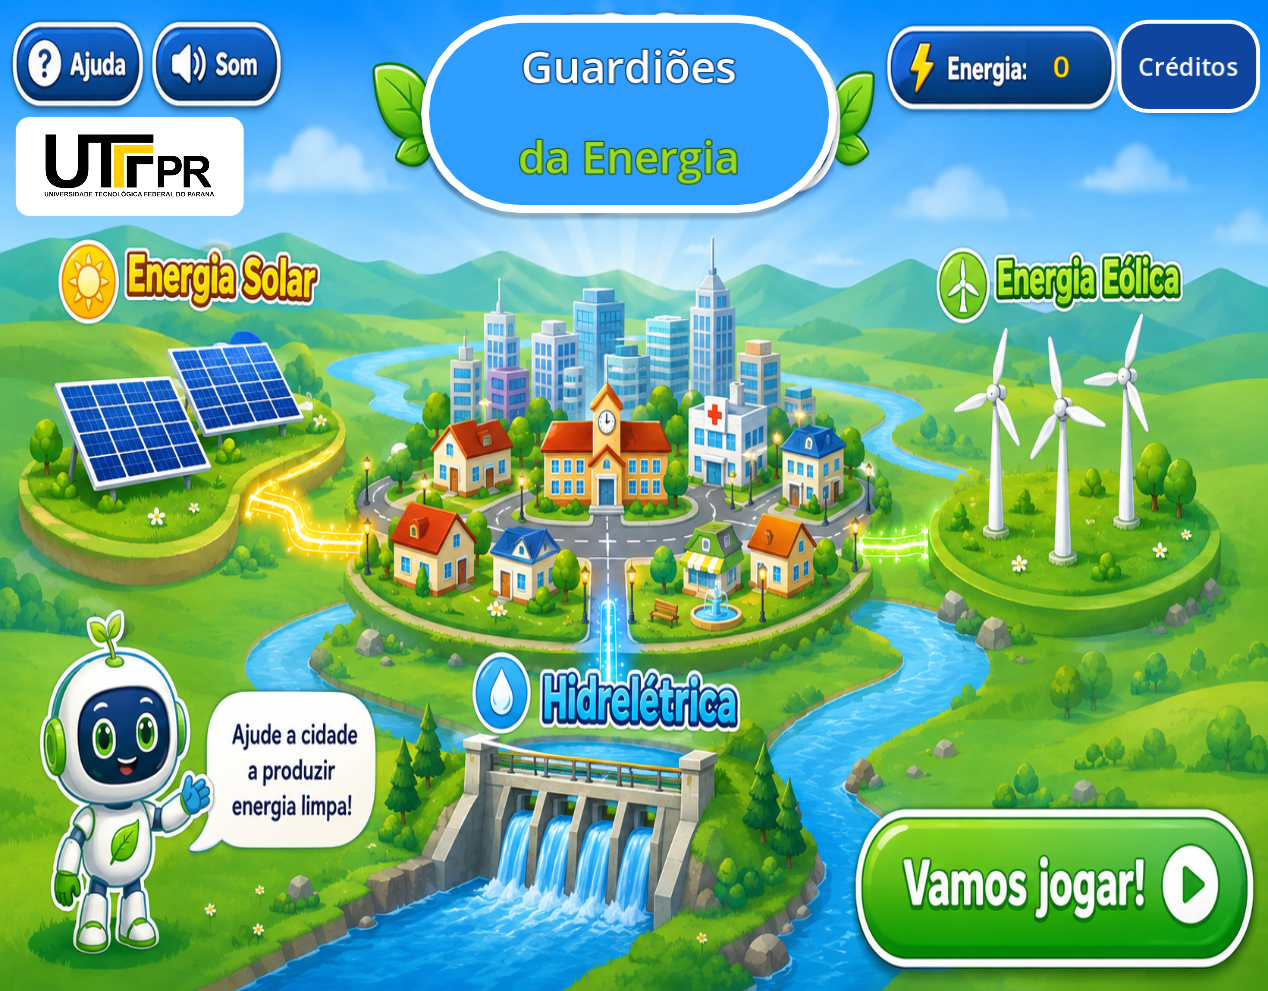
\includegraphics[width=0.75\textwidth]{figuras/menu_inicial.png}
\fonte{Autoria própria (2026)}
\end{figure}

Para conectar as fases, foi criada a história ``Cidade sem luz'': as três usinas da cidade pararam, e cada usina ligada devolve a energia a uma parte da cidade (as casas, a escola e as ruas). No modo de aventura completa, a história é contada pelo Tiko em quatro quadros de abertura (Figura~2), antes da primeira fase.

\begin{figure}[H]
\centering
\caption{Primeiro quadro da abertura da história}
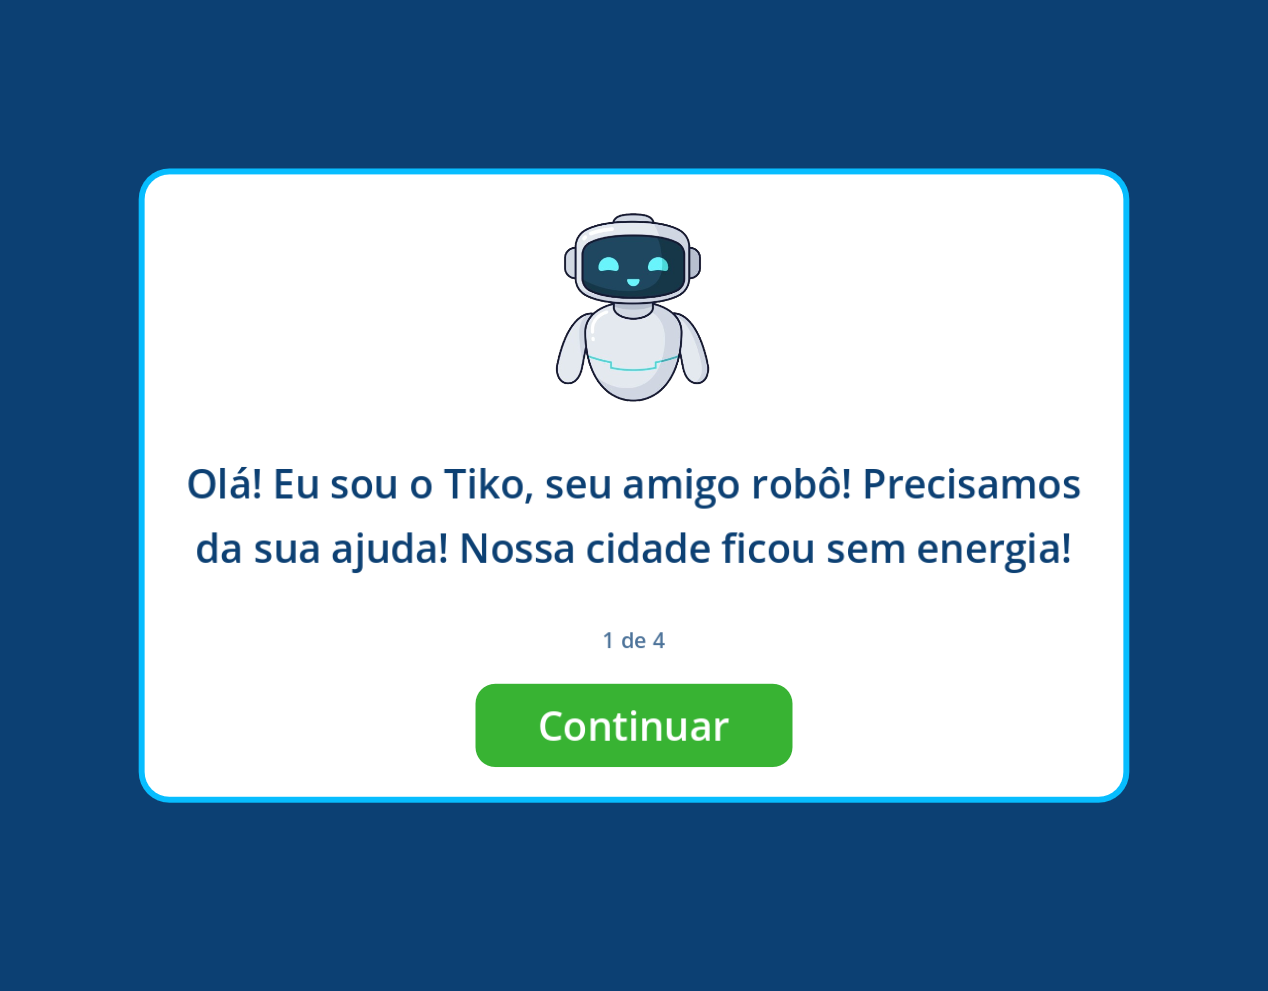
\includegraphics[width=0.6\textwidth]{figuras/abertura.png}
\fonte{Autoria própria (2026)}
\end{figure}

As três fases são descritas a seguir.

\begin{itemize}
\item \textbf{Usina Solar:} o jogador limpa 15 manchas dos painéis passando o mouse sobre elas. Depois, gira o painel do meio na direção do sol, com botões ou com as setas do teclado, e confirma. Isso se repete com o sol em três posições diferentes (Figura~3).
\item \textbf{Usina do Vento:} o vento alterna entre fraco e forte. Antes de cada rajada aparece o aviso ``VEM VENTO FORTE!'', e o jogador deve segurar o botão FREIO (ou a barra de espaço) durante a rajada e soltá-lo na calmaria, para produzir energia sem danificar a turbina. A fase dura 90 segundos (Figura~4).
\item \textbf{Usina da Água:} o jogador abre e fecha a comporta da represa para manter o nível da água na faixa ideal durante 60 segundos. O clima (sol, chuva ou tempestade) muda a quantidade de água que entra na represa (Figura~5).
\end{itemize}

\begin{figure}[H]
\centering
\caption{Fase da Usina Solar, etapa de limpeza dos painéis}
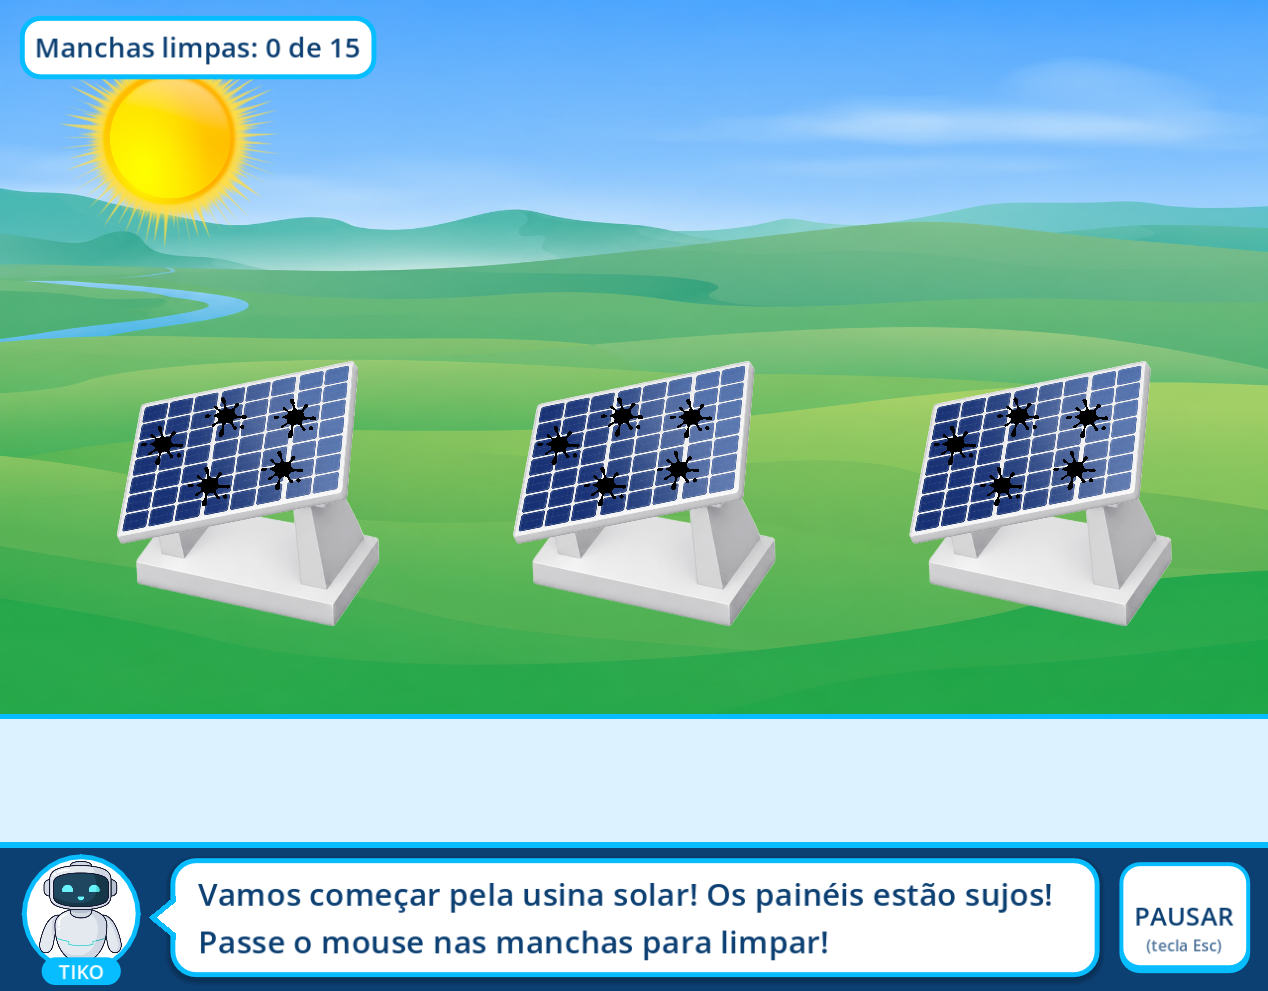
\includegraphics[width=0.6\textwidth]{figuras/fase_solar.png}
\fonte{Autoria própria (2026)}
\end{figure}

\begin{figure}[H]
\centering
\caption{Fase da Usina do Vento durante uma rajada}
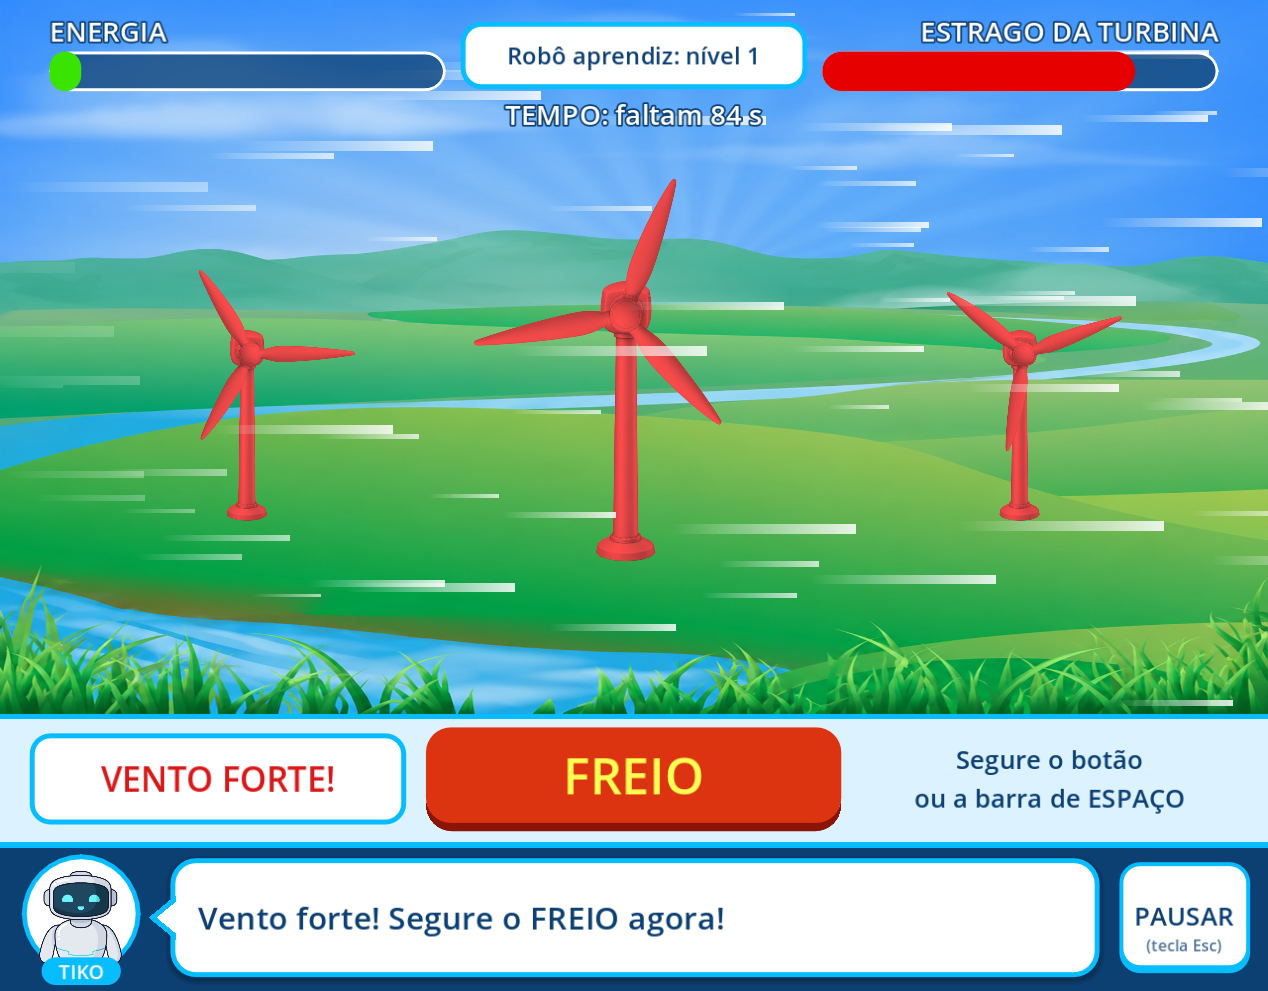
\includegraphics[width=0.6\textwidth]{figuras/fase_eolica.png}
\fonte{Autoria própria (2026)}
\end{figure}

\begin{figure}[H]
\centering
\caption{Fase da Usina da Água}
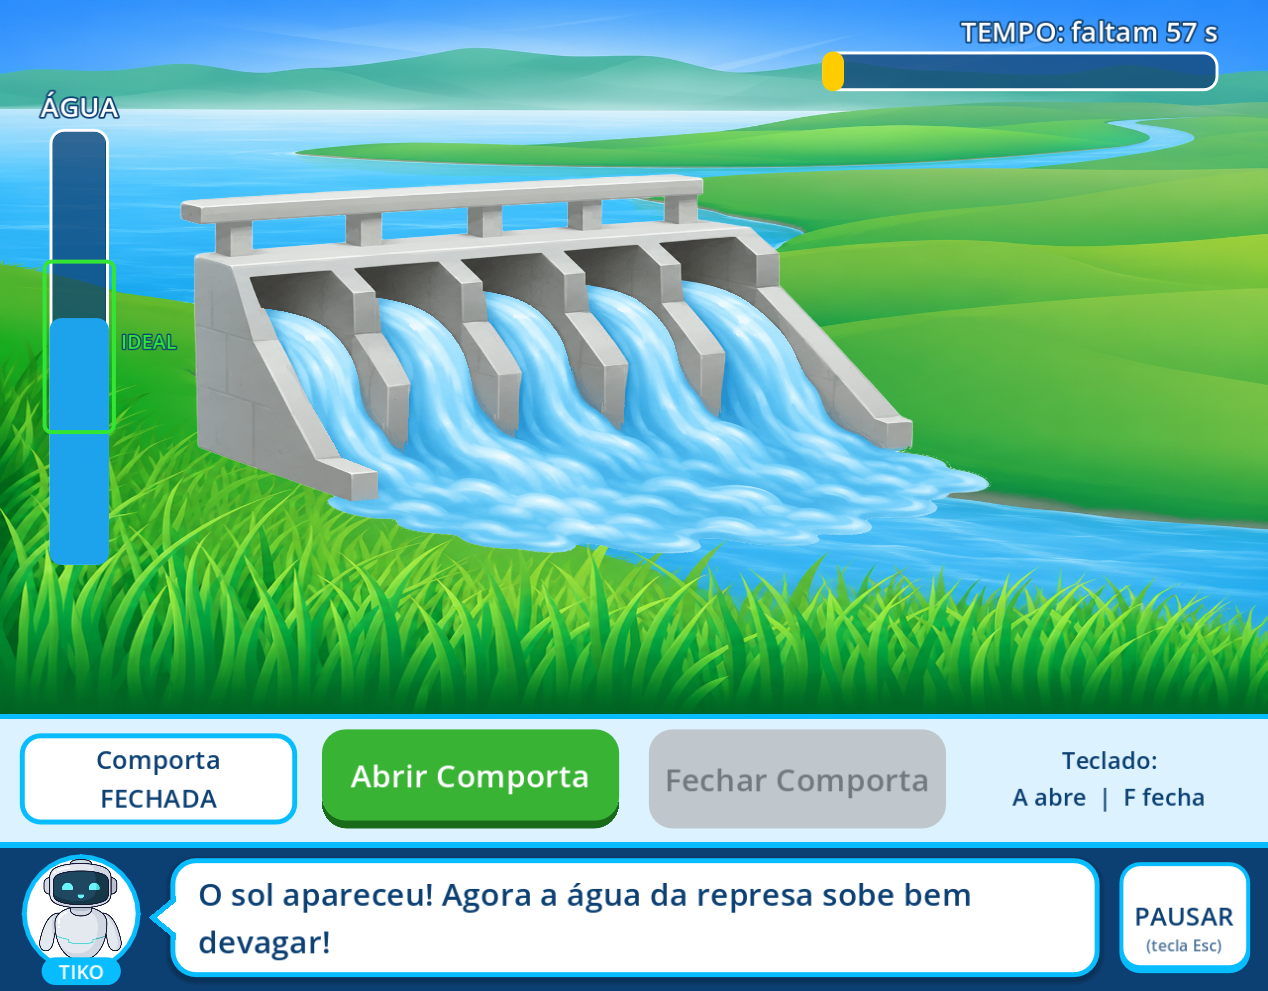
\includegraphics[width=0.6\textwidth]{figuras/fase_hidro.png}
\fonte{Autoria própria (2026)}
\end{figure}

Cada fase vale de 0 a 100 pontos. Na Usina Solar, cada alinhamento recebe uma nota que considera a precisão (até 7,5° de erro vale 100 pontos, e a nota cai até zero com 67,5° de erro) e o tempo (após 15 segundos, perde-se 2 pontos por segundo, no máximo 30). A pontuação da fase é $10 + 0{,}9 \times$ a média das três notas, em que os 10 pontos iniciais correspondem à limpeza dos painéis. Na Usina do Vento, a pontuação é a média do desempenho do jogador nas rajadas, multiplicada por 100 (Seção 2.2.2). Na Usina da Água, a pontuação é a porcentagem do minuto em que a água ficou na faixa ideal. No final, o jogador recebe três estrelas se a média das fases for 80 pontos ou mais, duas estrelas se for 50 ou mais, e uma estrela nos demais casos.

\subsection{Inteligências Artificiais das Fases}

Cada fase usa uma técnica de IA, apresentada ao jogador como o ``robô aprendiz''. Em todas elas, o aprendizado começa do zero a cada partida e não é salvo. A organização das IAs foi revisada durante o projeto, seguindo as orientações recebidas: o algoritmo de aprendizado foi separado das regras do jogo, a recompensa foi definida explicitamente, os estados terminais e os empates passaram a ser tratados, e as gerações da fase eólica passaram a acontecer durante a própria partida.

\subsubsection{Usina Solar: Q-Learning}

Na fase solar, o robô aprendiz aprende a virar os painéis para o sol com o algoritmo Q-Learning (Watkins; Dayan, 1992). O Q-Learning é um método de aprendizado por reforço: o agente experimenta ações, recebe recompensas e guarda em uma tabela Q o valor esperado de cada ação em cada estado (Sutton; Barto, 2018). A tabela é atualizada pela equação:

\begin{equation}
Q(s,a) \leftarrow Q(s,a) + \alpha \left[ r + \gamma \max_{a'} Q(s',a') - Q(s,a) \right]
\end{equation}

\noindent em que $s$ é o estado atual, $a$ é a ação escolhida, $r$ é a recompensa recebida, $s'$ é o novo estado, $\alpha = 0{,}2$ é a taxa de aprendizado e $\gamma = 0{,}9$ é o fator de desconto. O agente foi modelado da seguinte forma:

\begin{itemize}
\item \textbf{Estado:} a diferença entre o ângulo ideal (painel voltado para o sol) e o ângulo atual do painel, arredondada de 15 em 15 graus. O estado 0 significa painel alinhado e é o estado terminal.
\item \textbf{Ações:} girar $-15$°, ficar parado (0°) ou girar $+15$°.
\item \textbf{Recompensa:} $+100$ ao alinhar o painel; $-|e|-2$ ao girar sem alinhar; e $-|e|$ ao ficar parado, em que $|e|$ é o erro em graus no novo estado. O erro faz o agente preferir estados mais próximos do sol, e a penalidade de 2 desestimula movimentos desnecessários.
\item \textbf{Estado terminal:} ao alinhar, não há estado futuro, então o termo $\max Q(s',a')$ vale zero.
\item \textbf{Escolha da ação:} política $\varepsilon$-gulosa com $\varepsilon = 0{,}2$ durante o treino. Empates entre ações são resolvidos por sorteio.
\end{itemize}

O jogador participa do aprendizado fornecendo experiências, sem que o agente o imite. Cada giro do jogador e cada confirmação viram atualizações da tabela Q. Depois de cada uma das três rodadas, o agente treina sozinho por 100 episódios, explorando posições aleatórias do sol e do painel. Ao final, ocorre um teste: o sol vai para uma posição nova, diferente das usadas nas rodadas, e o robô gira os painéis sozinho, com $\varepsilon = 0$ (sem exploração). Em seguida, uma demonstração mostra o sol atravessando o céu e os painéis acompanhando seu movimento.

\subsubsection{Usina do Vento: Algoritmo Genético}

Na fase eólica, o robô aprendiz cria as rajadas de vento com um Algoritmo Genético (AG), técnica inspirada na evolução natural, em que uma população de soluções passa por seleção, cruzamento e mutação ao longo das gerações (Holland, 1975). Cada indivíduo é uma rajada descrita por quatro genes de valor real: força do vento (80 a 110), tempo de aviso antes da rajada (0,8 a 2,5 segundos), duração da rajada (1,5 a 3,0 segundos) e intervalo de calmaria depois dela (2,0 a 3,5 segundos).

A população tem quatro indivíduos, e cada um é testado ao vivo com o jogador, na sequência aviso, rajada e calmaria. O desempenho $d$ do jogador em cada rajada é calculado por:

\begin{equation}
d = 1 - 0{,}7\,e_r - 0{,}3\,e_c, \qquad e_r = \min\!\left(1, \frac{D}{40}\right), \qquad e_c = \min\!\left(1, \frac{t_f}{I}\right)
\end{equation}

\noindent em que $D$ é o estrago sofrido pela turbina durante a rajada, $t_f$ é o tempo em que o jogador freou na calmaria (perdendo energia) e $I$ é a duração da calmaria. A função de aptidão (\textit{fitness}) segue a ideia de ``desafio na medida'': as melhores rajadas são aquelas em que o jogador acerta quase tudo, mas não tudo. Por isso, a aptidão é maior quanto mais próximo o desempenho estiver de um alvo de 0,8:

\begin{equation}
f = \max\!\left(0{,}01,\; 1 - \frac{|d - 0{,}8|}{0{,}8}\right)
\end{equation}

Quando os quatro indivíduos são avaliados, uma nova geração é criada: os dois indivíduos com maior aptidão são escolhidos como pais; o melhor passa sem alteração para a próxima geração (elitismo); e os demais são gerados por cruzamento uniforme, em que cada gene vem de um dos pais com 50\% de chance. Depois, cada gene sofre mutação com 20\% de chance, sendo alterado em até 25\% da sua faixa de valores, sem ultrapassar os limites. O número da geração aparece na tela como ``Robô aprendiz: nível N'', e o Tiko avisa quando novos ventos são preparados.

\subsubsection{Usina da Água: Q-Learning do clima}

Na fase hidrelétrica, o robô aprendiz controla o clima, também com Q-Learning. O objetivo do agente é manter o jogo desafiador, mas jogável. A cada 5 segundos, o agente avalia a decisão anterior e escolhe um novo clima. O agente foi modelado da seguinte forma:

\begin{itemize}
\item \textbf{Estado:} combinação do nível da água (baixo, abaixo de 30; ideal, de 30 a 70; ou alto, acima de 70) com a situação da comporta (aberta ou fechada), totalizando seis estados.
\item \textbf{Ações:} sol, chuva ou tempestade. Por segundo, o sol acrescenta 2 unidades de água à represa, a chuva acrescenta 6 e a tempestade acrescenta 14. A comporta aberta retira 9 unidades por segundo.
\item \textbf{Recompensa:} $+10$ quando a água está na faixa ideal no momento da avaliação, $-5$ quando está fora dela e $-20$ quando a água transborda ou seca, o que encerra a fase. Esse último caso é tratado como estado terminal.
\item \textbf{Parâmetros:} $\alpha = 0{,}1$, $\gamma = 0{,}9$ e política $\varepsilon$-gulosa com $\varepsilon = 0{,}2$. Os empates são resolvidos por sorteio.
\end{itemize}

\subsection{Avaliação Experimental do Agente Solar}

Para verificar se o agente da fase solar realmente aprende, foi criado um experimento separado do jogo, que utiliza o mesmo código do agente. Foram testadas sete quantidades de episódios de treino (0, 30, 50, 100, 150, 200 e 250). Para cada quantidade, foram feitas 30 execuções independentes. Em cada execução, o agente treinado foi testado com $\varepsilon = 0$ em 100 combinações fixas de posição do sol e do painel. Mediu-se a taxa de sucesso (painel alinhado em até 15 passos), o erro médio final e o número médio de movimentos. Um segundo experimento variou a penalidade por girar (0, 2, 5 e 10), mantendo 100 episódios de treino.

\subsection{Adaptações para Pessoas com DI}

As decisões de interface seguiram as orientações apresentadas na Seção 1. Os pontos trabalhados foram:

\begin{itemize}
\item \textbf{Textos:} todas as 55 falas do Tiko foram reescritas em frases curtas e diretas e, depois, passaram por uma revisão de linguagem. As falas explicam o que está acontecendo e o que o jogador deve fazer. O tamanho da letra do balão se ajusta automaticamente para que o texto sempre caiba.
\item \textbf{Narração:} todas as falas foram gravadas com voz sintética na ferramenta ElevenLabs, com ritmo moderado (cerca de 145 palavras por minuto) e a mesma voz em todo o jogo. A voz toca junto com o texto do balão, e o jogo só avança quando ela termina.
\item \textbf{Tutoriais:} antes de cada fase, um painel mostra os passos numerados de como jogar (Figura~6), que também são lidos em voz alta. As dicas podem ser vistas de novo pelo menu de pausa.
\item \textbf{Áudio:} uma música de fundo instrumental, sem letra, toca em repetição e fica mais baixa enquanto o Tiko fala. O botão Som abre uma barra para ajustar o volume.
\item \textbf{Controles:} todas as ações podem ser feitas com o mouse ou com o teclado, com botões grandes e cores que indicam o estado (por exemplo, a barra de água fica laranja fora da faixa ideal).
\end{itemize}

\begin{figure}[H]
\centering
\caption{Tutorial da fase da Usina Solar}
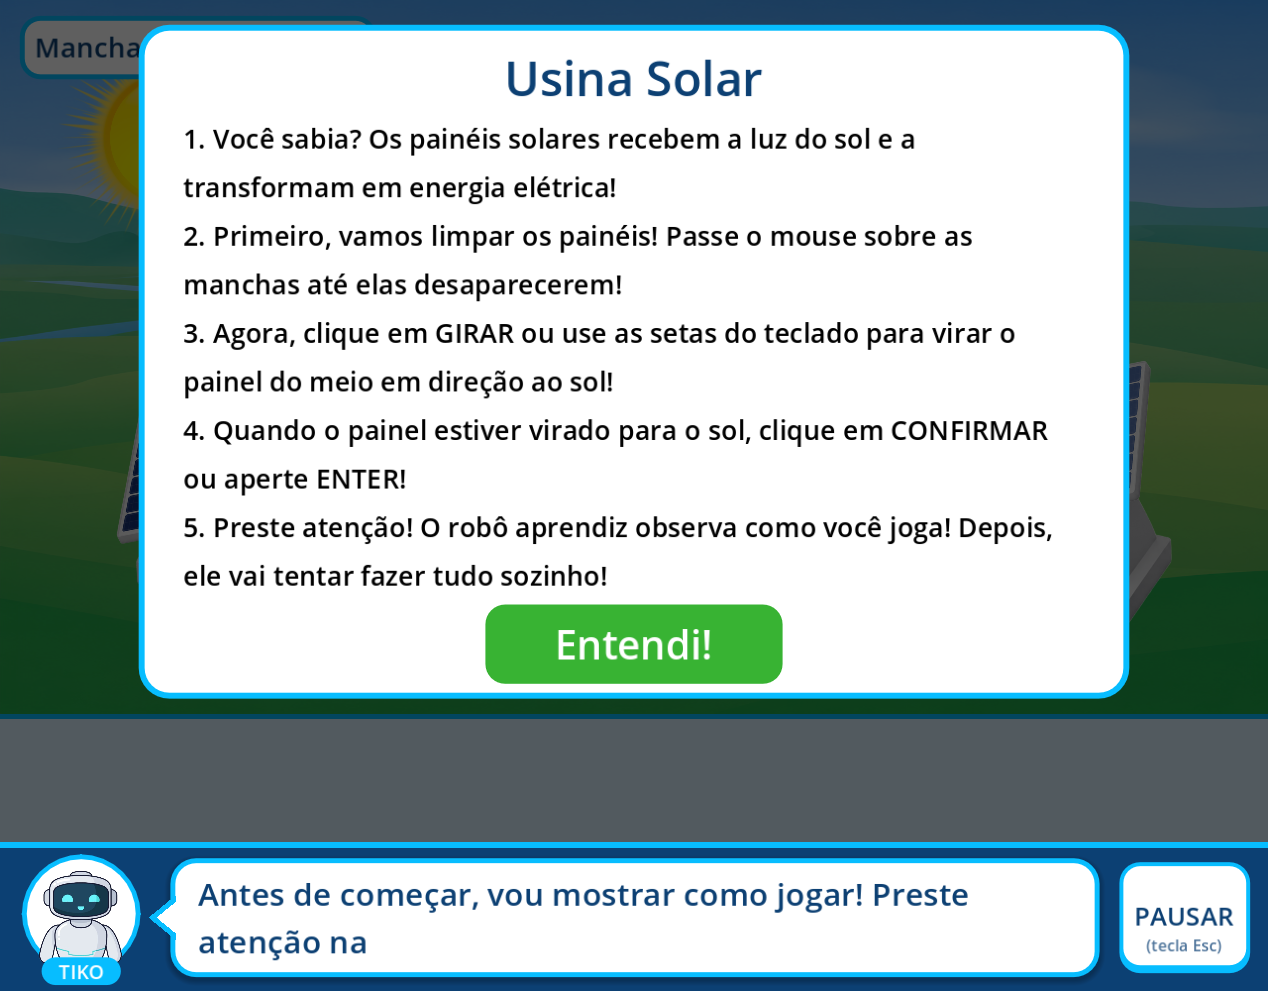
\includegraphics[width=0.6\textwidth]{figuras/tutorial_solar.png}
\fonte{Autoria própria (2026)}
\end{figure}

\subsection{Método de Avaliação do Jogo}

Para avaliar o jogo com os alunos, foram analisados três métodos: o MEEGA+, criado para o ensino superior (Petri; Gresse von Wangenheim; Borgatto, 2019); o MEEGA+KIDS, sua adaptação para a educação básica (Gresse von Wangenheim; Petri; Borgatto, 2020); e o SEGEM, criado para jogos sérios usados por pessoas com DI (Ribeiro, 2023). O SEGEM foi escolhido como base por ter sido desenvolvido e aplicado com alunos com DI leve e moderada. Ele recomenda poucas perguntas para os alunos e uma escala de apenas três opções, pois esse público tende a se cansar mais rapidamente em atividades teóricas (Ribeiro, 2023).

Com base nisso, foi elaborado um questionário curto para os alunos, com nome, idade e turma e 13 perguntas respondidas com ``Sim'', ``Mais ou menos'' ou ``Não''. As perguntas abordam a diversão, o desafio, a atenção, a facilidade de uso do mouse e do teclado, a compreensão das imagens e das regras, a autonomia, a ajuda da narração do Tiko e o aprendizado sobre as fontes de energia.

% ---------------------------------------------------------------------
\section{Resultados e Discussões}
% ---------------------------------------------------------------------

O jogo foi concluído com as três fases, a história de abertura, os tutoriais narrados, a música, o controle de volume, a tela de créditos e o logotipo da UTFPR no menu inicial. O resultado do experimento com o agente da fase solar está na Tabela~1 e na Figura~7.

\begin{table}[H]
\centering
\caption{Desempenho do agente solar conforme a quantidade de episódios de treino (30 execuções cada, penalidade por girar igual a 2)}
\begin{tabular}{cccc}
\toprule
Episódios & Taxa de sucesso (\%) & Erro médio (°) & Movimentos médios \\
\midrule
0   & 0,0 $\pm$ 0,0   & 60,68 & 0,00 \\
30  & 58,7 $\pm$ 10,0 & 41,40 & 2,81 \\
50  & 67,2 $\pm$ 6,9  & 36,83 & 2,79 \\
100 & 82,3 $\pm$ 3,6  & 24,14 & 3,38 \\
150 & 88,4 $\pm$ 4,5  & 18,01 & 3,70 \\
200 & 92,2 $\pm$ 2,8  & 13,94 & 3,83 \\
250 & 93,2 $\pm$ 2,6  & 12,79 & 3,82 \\
\bottomrule
\end{tabular}
\fonte{Autoria própria (2026)}
\end{table}

\begin{figure}[H]
\centering
\caption{Taxa de sucesso do agente solar em função dos episódios de treino}
\begin{tikzpicture}
\begin{axis}[
  width=0.75\textwidth, height=6cm,
  xlabel={Episódios de treino}, ylabel={Taxa de sucesso (\%)},
  xmin=0, xmax=260, ymin=0, ymax=100,
  xtick={0,30,50,100,150,200,250},
  ytick={0,20,40,60,80,100},
  grid=major, grid style={gray!25},
  tick label style={font=\small}, label style={font=\small},
]
\addplot[thick, mark=*, color=blue!70!black,
  error bars/.cd, y dir=both, y explicit]
  coordinates {
    (0,0) +- (0,0)
    (30,58.7) +- (0,10.0)
    (50,67.2) +- (0,6.9)
    (100,82.3) +- (0,3.6)
    (150,88.4) +- (0,4.5)
    (200,92.2) +- (0,2.8)
    (250,93.2) +- (0,2.6)
  };
\end{axis}
\end{tikzpicture}
\fonte{Autoria própria (2026)}
\end{figure}

Sem treino, o agente não acerta nenhum caso, pois todos os valores da tabela Q começam em zero e a escolha empatada favorece ficar parado. A taxa de sucesso sobe rapidamente até 100 episódios (82,3\%) e cresce mais devagar depois disso, chegando a 93,2\% com 250 episódios. O desvio padrão também diminui, o que indica que o agente fica mais consistente entre as execuções. O número médio de movimentos ficou abaixo do mínimo necessário para resolver todos os casos (4,05), porque as falhas ocorrem principalmente quando o agente para antes de alinhar. Na partida real, o agente recebe 300 episódios de treino (100 por rodada) e as experiências do jogador, o que corresponde à região de maior taxa de sucesso do experimento.

Os valores aprendidos se aproximaram dos valores teóricos. Por exemplo, quando falta um passo de 15° para alinhar, girar na direção certa leva ao estado terminal e vale $Q = 100$. Quando faltam dois passos, girar vale $-17 + 0{,}9 \times 100 = 73$, que foi o valor encontrado pelo agente. A Tabela~2 mostra o efeito da penalidade por girar.

\begin{table}[H]
\centering
\caption{Efeito da penalidade por girar (100 episódios de treino, 30 execuções cada)}
\begin{tabular}{cccc}
\toprule
Penalidade & Taxa de sucesso (\%) & Erro médio (°) & Movimentos médios \\
\midrule
0  & 83,3 $\pm$ 5,4 & 23,16 & 3,49 \\
2  & 82,3 $\pm$ 3,6 & 24,14 & 3,38 \\
5  & 81,0 $\pm$ 4,3 & 25,55 & 3,36 \\
10 & 80,0 $\pm$ 6,6 & 25,86 & 3,11 \\
\bottomrule
\end{tabular}
\fonte{Autoria própria (2026)}
\end{table}

Penalidades maiores reduzem o número de movimentos, mas também reduzem um pouco a taxa de sucesso, pois o agente passa a evitar giros mesmo quando eles seriam úteis. A penalidade 2, usada no jogo, mantém a taxa de sucesso próxima da obtida sem penalidade.

Na fase eólica, um teste com um jogador simulado mostrou que, nos 90 segundos de partida, ocorrem cerca de 14 rajadas e quatro gerações do AG. Assim, o jogador percebe a evolução do robô aprendiz durante a partida. Nesse teste, a população tendeu a reduzir o tempo de aviso, tornando as rajadas mais difíceis à medida que o jogador acertava. Como a população é pequena (quatro indivíduos) e usa elitismo, ela perde diversidade rapidamente, o que limita a variedade de rajadas em partidas longas.

Na fase hidrelétrica, cada partida tem cerca de 12 decisões do agente (uma a cada 5 segundos durante 60 segundos). Esse número é pequeno para que a tabela Q convirja dentro de uma única partida. Nos testes, o agente tendeu a escolher o sol com mais frequência, pois esse clima facilita manter a água na faixa ideal, que é a situação recompensada.

Não foi possível, até o momento, aplicar o jogo e o questionário com os alunos da instituição parceira. Por esse motivo, os resultados sobre acessibilidade baseiam-se nas orientações da literatura e nas revisões feitas com a orientadora, e não em dados de uso. Essa é a principal limitação do trabalho.

% ---------------------------------------------------------------------
\section{Conclusão}
% ---------------------------------------------------------------------

Este trabalho teve como objetivo desenvolver o jogo educacional ``Guardiões da Energia'', que ensina as fontes de energia solar, eólica e hidrelétrica a pessoas com DI e utiliza uma técnica de IA diferente em cada fase. O jogo foi desenvolvido no Godot 4.5, com uma história que conecta as fases e com o personagem Tiko guiando o jogador por meio de falas curtas e narradas.

As IAs foram implementadas e revisadas conforme as orientações recebidas: Q-Learning para alinhar os painéis na fase solar, com o jogador fornecendo experiências ao agente; Algoritmo Genético para criar rajadas de vento com ``desafio na medida'' na fase eólica, com as gerações acontecendo durante a partida; e Q-Learning para controlar o clima na fase hidrelétrica. O experimento com o agente solar mostrou que a taxa de sucesso passa de 0\% sem treino para 93,2\% com 250 episódios, confirmando que o agente aprende. A interface foi adaptada com textos curtos, narração, tutoriais, controle de volume e controles simples. Além disso, foi elaborado um questionário de avaliação baseado no método SEGEM.

A principal limitação do trabalho foi a ausência de validação com os alunos da instituição parceira. Como trabalhos futuros, pretende-se aplicar o jogo e o questionário na instituição parceira; publicar a versão para navegador; aumentar a diversidade da população do AG da fase eólica; ampliar o número de decisões do agente da fase hidrelétrica para que ele aprenda mais em cada partida; e incluir recursos de acessibilidade como um botão para repetir a última fala, legendas sincronizadas com a narração e elogios variados.

% ---------------------------------------------------------------------
\newpage
\section*{REFERÊNCIAS}
% ---------------------------------------------------------------------
\begingroup
\singlespacing
\setlength{\parindent}{0pt}
\setlength{\parskip}{10pt}

GRESSE VON WANGENHEIM, C.; PETRI, G.; BORGATTO, A. F. MEEGA+KIDS: a model for the evaluation of games for computing education in secondary school. \textbf{RENOTE -- Revista Novas Tecnologias na Educação}, Porto Alegre, v. 18, n. 1, 2020.

GUSMÃO, E. C. R.; MATOS, G. S.; ALCHIERI, J. C.; CHIANCA, T. C. M. Habilidades adaptativas sociais e conceituais de indivíduos com deficiência intelectual. \textbf{Revista da Escola de Enfermagem da USP}, São Paulo, v. 53, e03481, 2019. DOI: 10.1590/S1980-220X2018014903481.

HOLLAND, J. H. \textbf{Adaptation in natural and artificial systems}. Ann Arbor: University of Michigan Press, 1975.

KUO, H. J.; YEOMANS, M.; RUIZ, D.; LIN, C.-C. Video games and disability: a risk and benefit analysis. \textbf{Frontiers in Rehabilitation Sciences}, v. 5, 1343057, 2024. DOI: 10.3389/fresc.2024.1343057.

PETRI, G.; GRESSE VON WANGENHEIM, C.; BORGATTO, A. F. MEEGA+: um modelo para a avaliação de jogos educacionais para o ensino de computação. \textbf{Revista Brasileira de Informática na Educação}, v. 27, n. 3, p. 52-81, 2019.

RIBEIRO, T. L. S. \textbf{Método de avaliação de jogos sérios}. 2023. Trabalho de Conclusão de Curso (Bacharelado em Ciência da Computação) -- Universidade Tecnológica Federal do Paraná, Ponta Grossa, 2023.

SEEMAN, L.; MONTGOMERY, R.; LEE, S.; RAN, R. (ed.). \textbf{Making content usable for people with cognitive and learning disabilities}. W3C Working Draft, 17 jul. 2020. Disponível em: \url{https://www.w3.org/TR/2020/WD-coga-usable-20200717/}. Acesso em: 16 nov. 2026.

SUTTON, R. S.; BARTO, A. G. \textbf{Reinforcement learning}: an introduction. 2. ed. Cambridge: MIT Press, 2018.

WATKINS, C. J. C. H.; DAYAN, P. Q-learning. \textbf{Machine Learning}, v. 8, n. 3-4, p. 279-292, 1992. DOI: 10.1007/BF00992698.

\endgroup

% ---------------------------------------------------------------------
% ASSINATURAS
% ---------------------------------------------------------------------
\vspace{3cm}
\begin{center}
\rule{8cm}{0.4pt}\\
Gabriel Jose Monteiro

\vspace{2.5cm}
\rule{8cm}{0.4pt}\\
Helyane Bronoski Borges
\end{center}

\end{document}
